\documentclass[a4paper,11pt]{article}
\usepackage[utf8]{inputenc}
\usepackage[T1]{fontenc}
\usepackage[english]{babel}
\usepackage{array}
\usepackage{multirow}
\usepackage{multicol}
\usepackage{fullpage}
\usepackage{listingsutf8}
\usepackage{caption}
\usepackage{float}
\usepackage{subcaption}
\usepackage{amsmath}
\usepackage{enumitem}
%%\usepackage{titling}
\usepackage{amsthm}
\usepackage{amsfonts}
\usepackage{amssymb}
\usepackage{color}
\usepackage{todonotes}
\usepackage[nounderscore]{syntax}
\usepackage{graphicx}
\definecolor{mygreen}{rgb}{0,0.6,0}
\definecolor{mygray}{rgb}{0.5,0.5,0.5}
\definecolor{mymauve}{rgb}{0.58,0,0.82}
\usepackage[hidelinks]{hyperref}

\newcommand\bb{Benjamin Boisson}
\newcommand\gc{Guillaume Combette}
\newcommand\dl{Dimitri Lajou}
\newcommand\vl{Victor Lutfalla}
\newcommand\om{Octave Mariotti}
\newcommand\mr{Raphaël Monat} % Okay, \rm was already taken too.
\newcommand\me{Etienne Moutot} % He is not the only one author o/ Just that \em is already taken
\newcommand\js{Johanna Seif}
\newcommand\ps{Pijus Simonaitis}



\title{Final report, Blend'it project}
\author{\bb, \gc, \dl,\\ \vl, \om\footnote{was abroad during the second semester, he did not contributed to the second part of the project}, \mr,\\ \me, \js, \ps}
\date{2015-2016}


\begin{document}

\pagenumbering{gobble}
\maketitle

\begin{figure}[h!]
\centerline{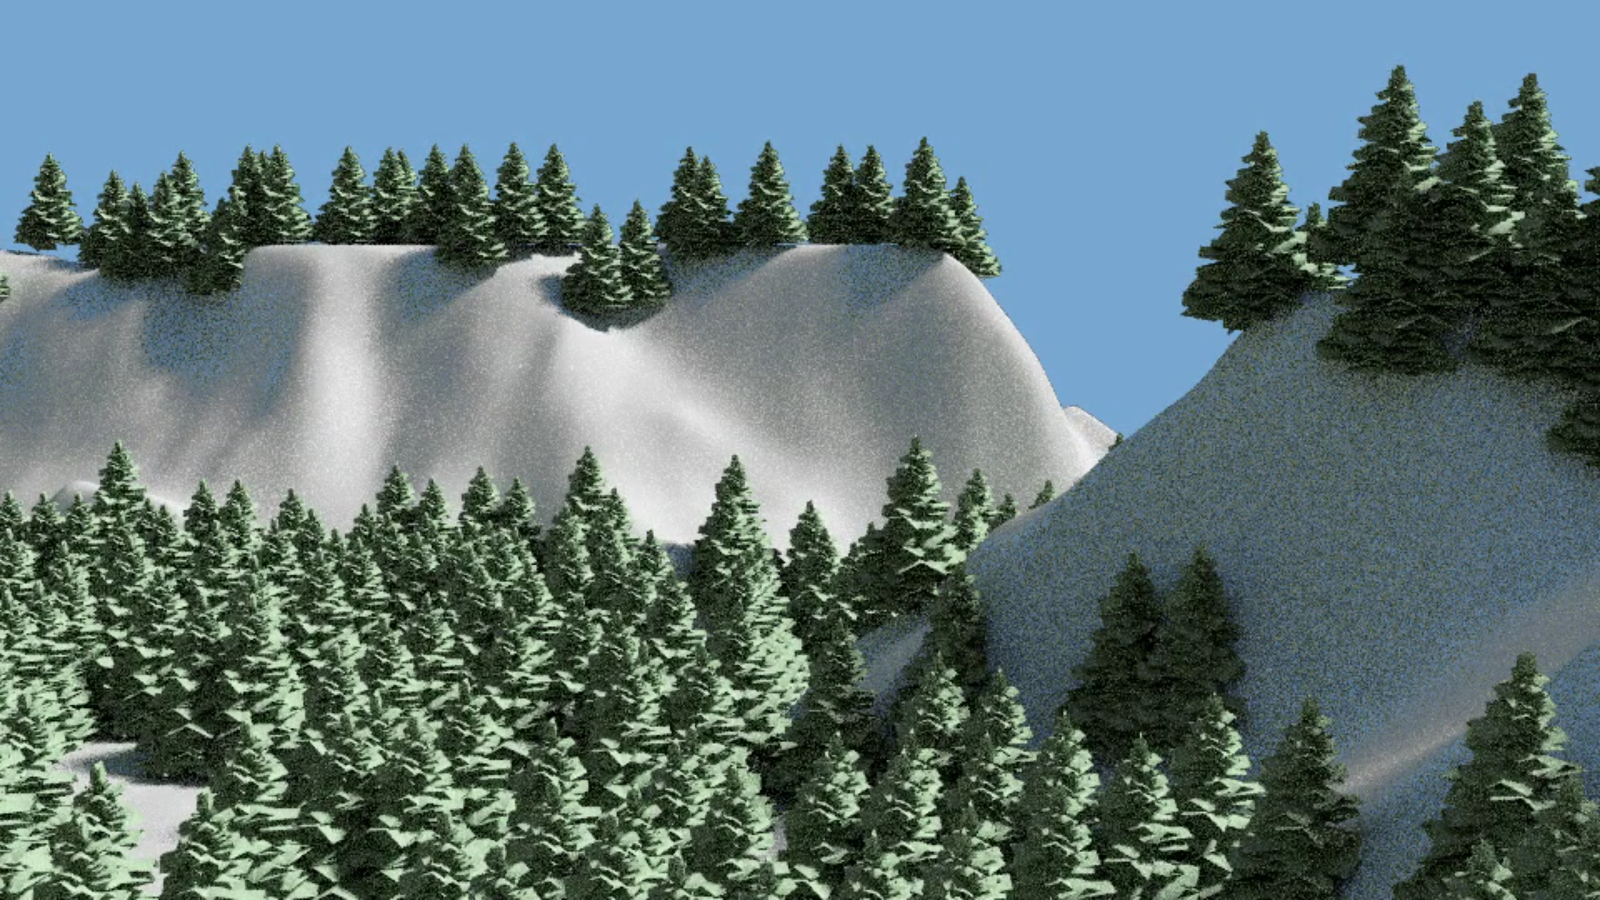
\includegraphics[scale=0.3]{img/demo.png}}
\end{figure}
%%\vspace{12cm}
\begin{abstract}
The goal of this project, ``Blend'it'', was to design two open-source plug-ins for Blender, which is a computer graphics software. These two plug-ins aim to help artists creating complex environments. The first of these plug-in should be able to realistically animate crowds, and the other one to design static environments by making different elements such as rivers and mountains automatically interact to produce realistic scenes. \\
Although this kind of software is already developed in the Computer Graphics industry, there are often unavailable to the public and not free.
\end{abstract}

\newpage
\pagenumbering{arabic}

\tableofcontents

\newpage

\section{Introduction}

\subsection{Objectives}

Blender is a complete open source 3D sofware, and can create 3D scenes from
scratch, from modeling to animation and rendering. The goal of this
project is to improve Blender, by
providing two new plug-ins to help artists creating rich environments.

Our aim is to add to Blender the possibility to generate large,
crowded environments. There are two independents parts: first
generate environments in a semi-automated way. Secondly, generate and
animate people in the environment. People's movements must be consistent
with the environment and other people's movements. There are some
examples of what has been created by some researchers in figures
\ref{fig:crowd} and \ref{fig:env}.

\begin{figure}[h] \centering

  \begin{subfigure}[t]{0.5\textwidth}
    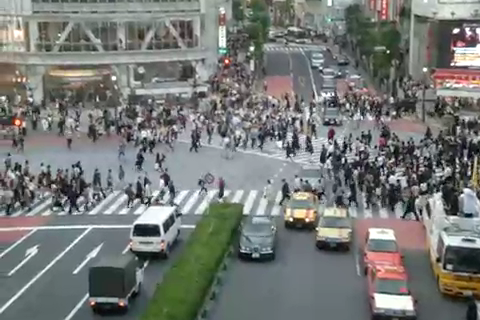
\includegraphics[width=7.5cm]{img/PLE_real.png}
    \caption{Real picture}
  \end{subfigure}% ~
  \begin{subfigure}[t]{0.5\textwidth}
    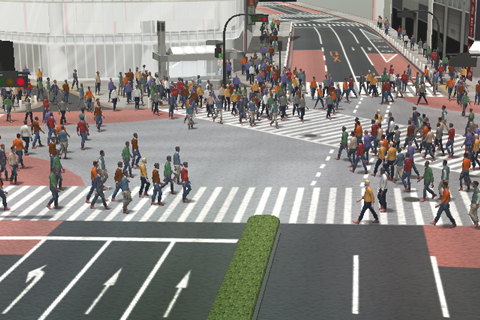
\includegraphics[width=7.5cm]{img/PLE_simu.png}
    \caption{Animation example from \cite{PLE}}
  \end{subfigure}
  \caption{A crossing in Tokyo}
  \label{fig:crowd}
\end{figure}

Note that Blend'it does not aim to be a realistic crowd generator, in
the sense of a usable simulator for sociological or scientific
experiments. The goal is to provide a complete generator for crowd and
environment for an artistic purpose only, that \textit{looks like} a
realistic crowd.

\begin{figure}[h]
  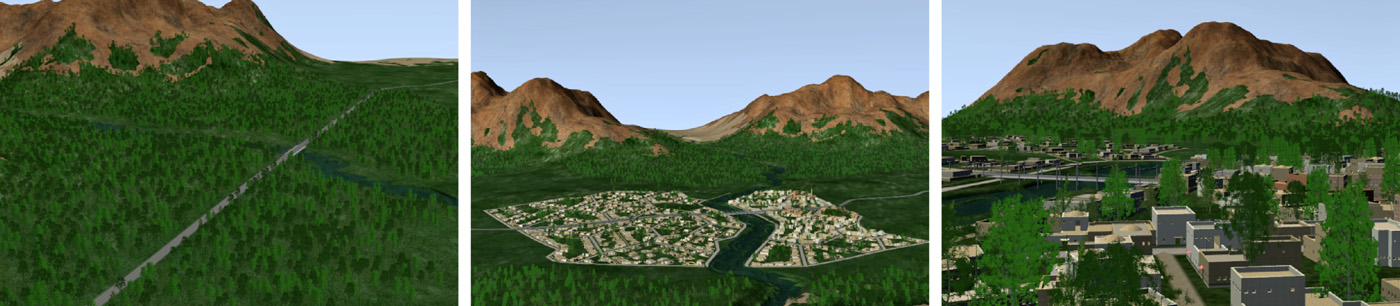
\includegraphics[width=15cm]{img/env1.jpg}
  \caption{Image taken from \cite{DeclarativeArchitecture}}
  \label{fig:env}
\end{figure}


There have been a lot of researches around the procedural generation
of crowds and environments in computer graphics. But the large
majority are implemented as research prototypes or in commercial
software. To the best of our knowledge, nothing exists for widely used
free software like Blender. 3D graphics is a domain that is still
closed-source, and every professional 3D artist uses costly
software. We think it is an important point to move some proprietary
technologies to the open-source world, to fill a little bit the gap.

\subsection{State of the art}

%% Reprendre remarque de l'expert : je crois que Massive est pas issu d'ilm ou un truc du genre
%% Reprendre des images du beamer ?


Animation of large crowds is really developed in the computer graphics
industry, enabling commercial 3D software to easily render massive
scenes with large crowds. For example, a software called Massive
(\cite{Massive}, Fig.~\ref{fig:massive}) dramatically changed the
habits of 3D studios: it helped generating the armies being displayed
in \textit{Lord of the Rings}. The Golaem software (\cite{Golaem},
Fig.~\ref{fig:golaem}) is also able to render massive crowds
in different situations, and is used by the studio producing
\textit{Game of Thrones}. Nowadays, even commercial standalone 3D
software like 3DS MAX \cite{3dsmax} is able to generate realistic
crowds. VUE is a software able to generate massive, realistic
landscapes, as presented in Fig.~\ref{fig:vue}. However, these software are really
expensive: Massive costs up to \$16,000 per year, and Golaem \$5000
per year. On the contrary, no open-source software provides this
kind of feature. In the past, scripts had been developed, but they
were not providing realistic results, and are not working anymore.


\begin{figure}[h] \centering
  \begin{subfigure}[t]{0.5\textwidth}
    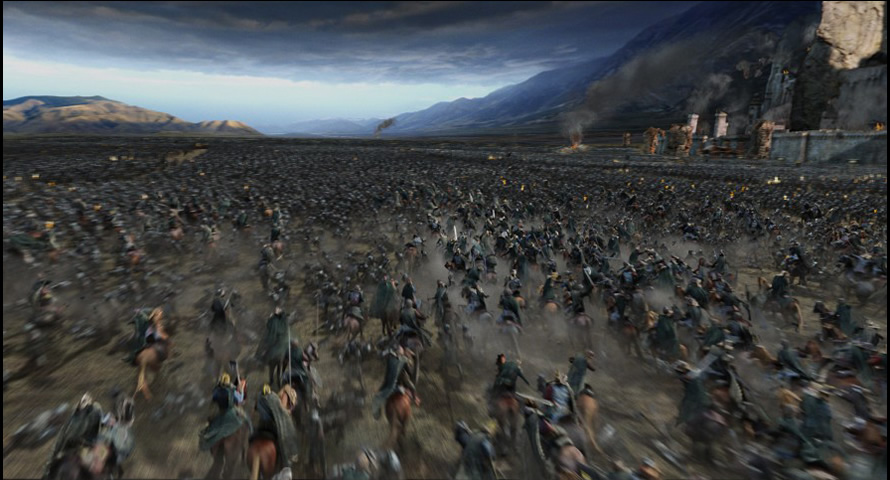
\includegraphics[width=0.9\textwidth]{img/massive.jpg}
    \caption{Scene generated using Massive}
    \label{fig:massive}
  \end{subfigure}% ~
  \begin{subfigure}[t]{0.5\textwidth}
    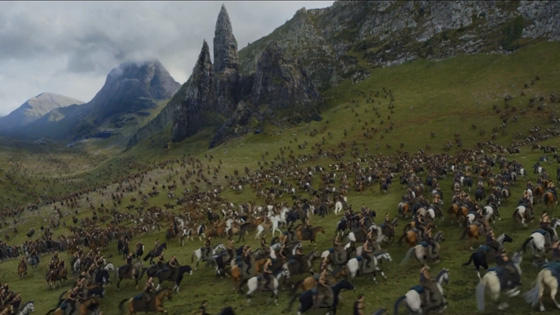
\includegraphics[width=0.9\textwidth]{img/golaem.jpg}
    \caption{Scene generated using Golaem}
    \label{fig:golaem}
  \end{subfigure}
  \caption{State-of-the-art crowd generation and animation}
  \label{fig:mg}
\end{figure}


\begin{figure}[h] \centering
  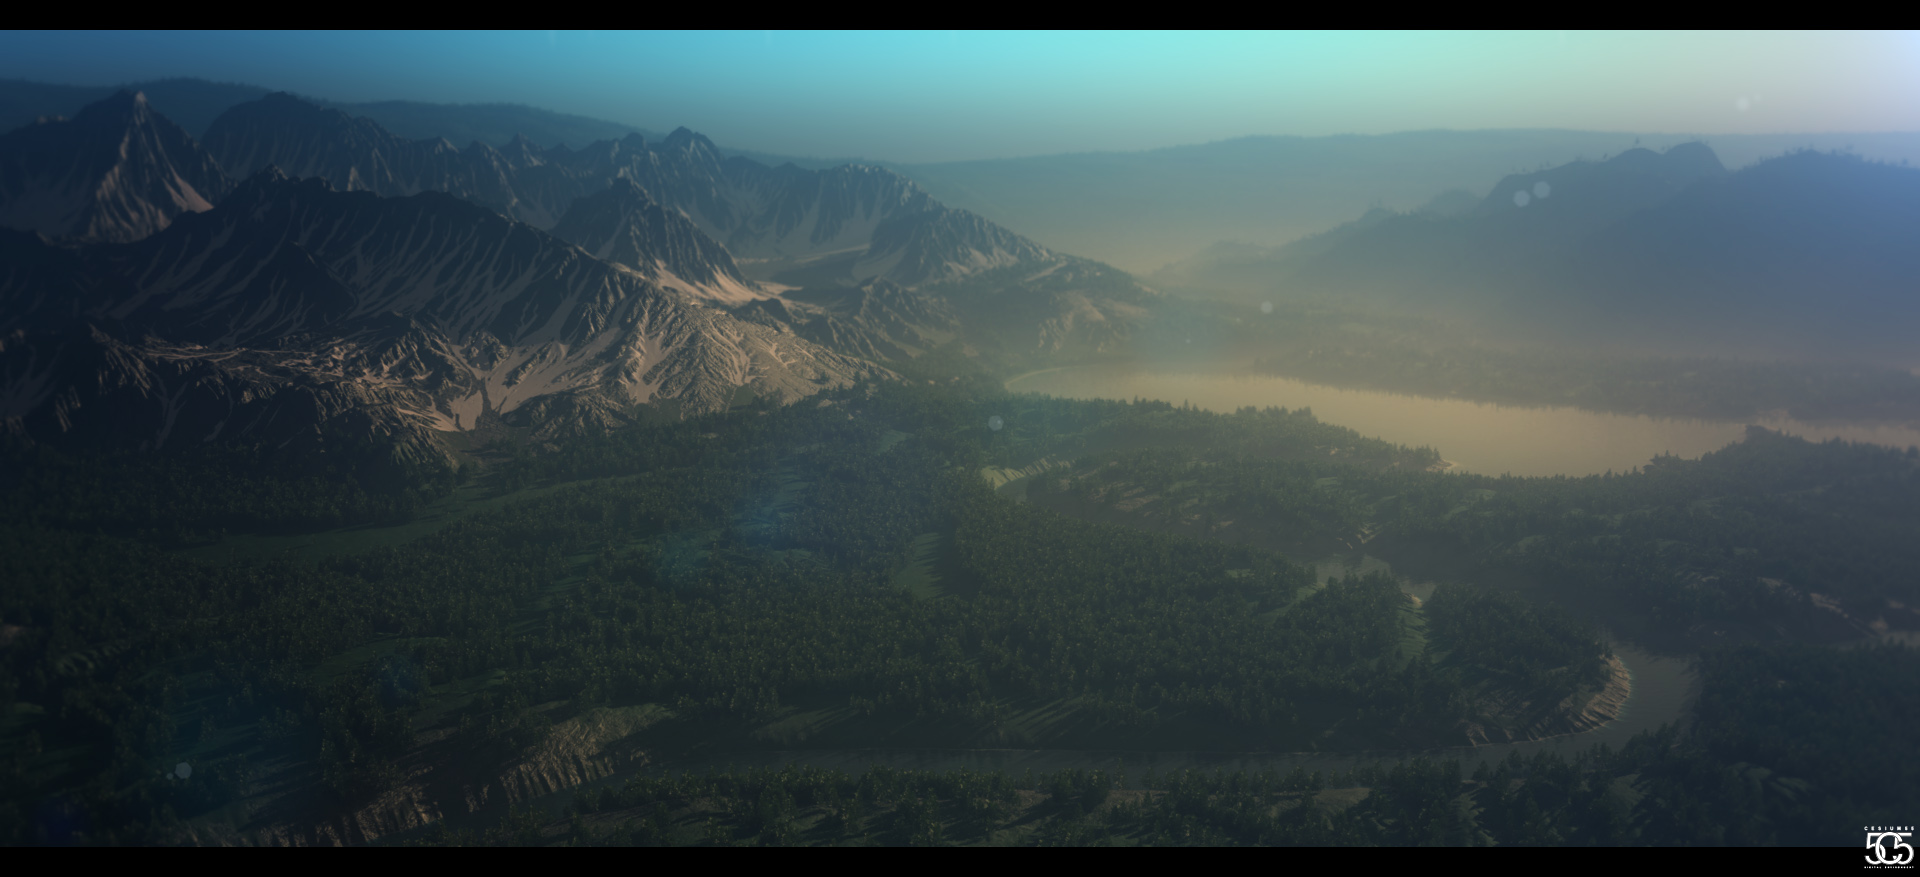
\includegraphics[width=0.95\textwidth]{img/vue.jpg}
  \caption{State-of-the-art landscape generation using VUE software}
  \label{fig:vue}
\end{figure}


\subsection{Team}

We are 9 Master students from the \textit{École Normale Supérieure de
Lyon}, France. As a part of our First year of Master in Research in
Computer Science, we need to develop and code a project of our choice
(here, ``Blend'it''), during the whole year. We are supervised by an
Associate Professor from the ENS Lyon, Eddy Caron. There is a project
leader, \me, and a deputy leader, \mr. Please do not hesitate to
contact us, by writing an email at \\
\textit{first name . last name@ens-lyon.fr}.


All our work is hosted on Github, and can be consulted on
\url{github.com/blendit}. We also have a website:
\url{blendit.github.io}.


\subsection{Choice of Blender.}

The big advantage of producing a code based on Blender is that we can
use its Python API, which is very powerful. With it, one can
manipulate every objects and part of the Blender interface without
re-compiling Blender or even modifying the source code. Thus, we can
concentrate only on the new parts of the project, that is our algorithms. We
did not need to code another render engine for example.  The other
advantage is the already existing Blender community on which
we can rely to have some feedback on our project.


\subsection{Structure of the project}

The two plug-in are currently independent, one is able to simulate the
motion of crowds, and one is able to generated environments. In each
plug-in, we split our code into a ``pure'' part, independent of
Blender, and one interacting with the Python API of Blender. This has
two advantages: we can test the ``pure'' part easily (testing the
Blender plug-in automatically is more difficult), and we may code
interface with other softwares too.



\paragraph{Outline}

\begin{itemize}
  \item In section 2, we present the work of the Blender exploration team, done by \mr, \me\ and \ps.
  \item Section 3 presents the work done by \dl, \vl,
\js\ and \ps \ on the crowd simulation.
 \item Section 4 presents the environment
plug-in, done by \bb, \gc, \mr\ and \me.
\item Section 5 concludes this report.
\end{itemize}

  

\newpage

\section{Blender exploration team}

During the whole project, this team had two aims. Our first goal was
to discover Blender and Python while other teams focused on the
bibliographical work, to then teach everyone how to use Blender
efficiently and code in Python. Our second goal was to guarantee the
quality of our code by setting up unitary tests and code coverage
tools.

\subsection{Blender discovery}

Blender is written in C++ and Python, but it has a powerful API in
Python, so we did not have to modify the C++ core of Blender. Blender
is also able to show the Python source of its interface, or give the
Python command associated to a manual operation. These features were
really helpful to develop efficiently our programs.


\subsection{Unitary tests}

For each new class we implemented, we also created a unit test
file. The execution was handled by the unitary test library of
Python. We linked our Github repositories with Travis, a website
that runs the tests every time a pull request is created.

The advantage of creating these tests is that it forced us to test
deeply our code, and more importantly, to notice when code modifications
break some other parts of the code. This last feature is really
important for big projects, to avoid creating bugs when modifying the
code.

\subsection{Code coverage}

We also linked our Github repositories with Coveralls, to see what
part of the code was covered by our unitary tests. To ensure a good
coverage, the pull requests had to increase coverage, or they would
automatically be rejected.

\subsection{Code organization}
%% TODO un peu redondant avec "structure of the project" dans intro ? 
This team also organized globally the code of the project. The code of
each plug-in is separated into two parts: one independent from
Blender, containing the \textit{core}, that is, the main algorithms
and data structures. The second part implements the interface with
Blender.


The advantage of this organization is that the first part can be
tested automatically using unit tests. The part using Blender cannot
be tested automatically with Travis, because it needs a lot of
interaction with the graphical interface. Thus, we tried to put
maximum of the complex algorithm in the first part, to allow them to
be tested extensively.

\begin{figure}[h]
  \begin{center}
    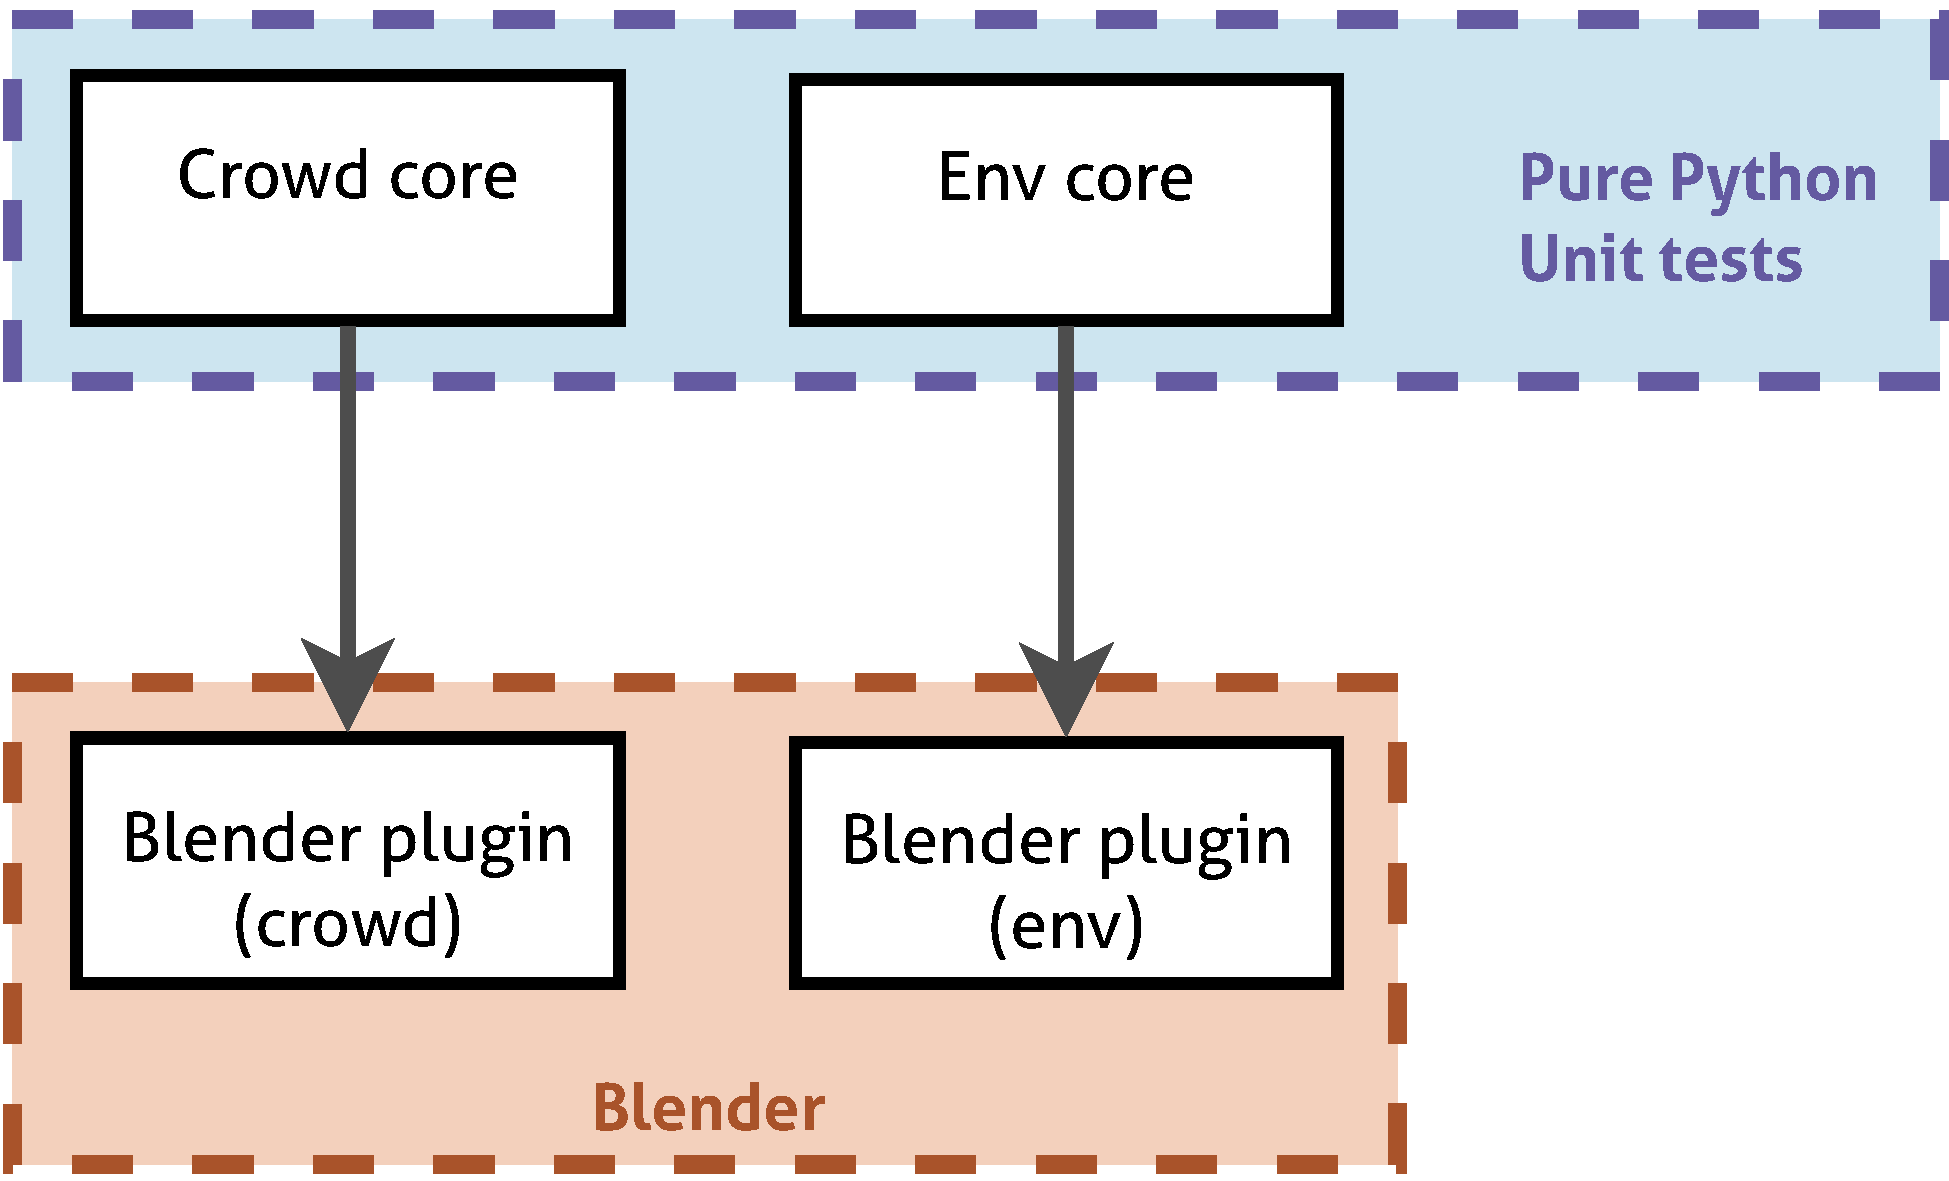
\includegraphics[width=7cm]{img/orga.pdf}
    \caption{Code organization}
    \label{fig:code}
  \end{center}
\end{figure}

\clearpage

\section{Crowd plug-in}

The goal of this work package was to implement an efficient and
realistic motion of a crowd.


The initial goal was to implement two parts: one creating trajectories
for the crowd and another one for animating individual movements. The
second part was really hard to implement and was closely linked with
the animation of models, which is a domain where we did not have any
expertise. We thus decided to focus on the first part.


Our code is split into two parts: one that is independent from Blender
and one that depends on it (see figure \ref{fig:code}).


The first part create a set of key points that will represent the
movement of one person and the second interpolate a trajectory from
those points. Before presenting these two parts, we explain the
difficulties encountered when we tried to model human animation.


\subsection{Human animation}

At the beginning we considered animating Humans and started by
analyzing a theoretical survey of computer animation of Human walking
(\cite{th_walking}) and looking for what was already done in Blender
concerning automatic walking. All Blender-related resources on walking
animation are gathered on a web-page
(\cite{blwikiwalking}). Walk-o-matic and stride add-ons were used in
previous versions of Blender to ``help to interactively design rough
passes of a walk'' and ``quickly create cycles for background or extra
characters'', however both were broken on Blender 2.7 and we are using
Blender 2.76.

Due to the lack of existing tools concerning automatic walking we
considered creating such a tool ourselves. We started by analyzing
tutorials on blender character animation (for example
\cite{tuto_walk}) and creating such a motion manually. However we soon
realized how difficult it is to generate a realistic walk due to the
complex physics behind the movements and decided that it is out of the
scope of our project. We have shifted our attention to the more basic
task of creating a path in Blender and making an object following it
with varying speed given by our algorithm.


% Il faudra changer les titres je pense
\subsection{Path generation}

The first algorithm is inspired by those two papers: \cite{PLE} and
\cite{vandenBerg2011}. We chose them because the notions involved in
the description of the algorithm were more familiar to us.  % TODO :
combler avec du bla bla The idea is the following: a graph (grid)
algorithm will generate a general path for each individual and another
algorithm will prevent collisions between individuals. \\ Time is
discretized, and for each time, we compute the direction to go for
each individual. We move the in this direction, and iterate this
principle. This is how we get the final set of points for each
individuals.


\subsubsection{Implementation}

%% Expliquer les parties avant de se lancer ?

\paragraph{The guide graph}

The first part that we tried to implement was the data structure of
the graph. We created a data structure representing the nodes of the
graph and the edges. This was quite easy to do since the graph is
supposed to be a grid, it is regular.  Then we needed a minimum
distance (1 to 1) algorithm on the graph. For that we chose the $A^*$
algorithm. Unfortunately, our implementation of the $A^*$ was really
costly in time and even more in memory. This fact forced us to abandon
the graph in the rest of the development. We could test it for small
values, and for a small number of calls, but the $A^*$ procedure would
have to be called thousands of times which makes this impractical.  To
replace the graph we used the euclidean distance, this involved
removing static obstacles (\textcolor{red}{TODO: pourquoi?}). Also the
points (representing people) were not  able to avoid packed places
anymore and just went strait to there goal.

\paragraph{Allowed velocity field}

This part deals with collision avoidance. This part is the part that
took us the more time to implement. The problem is the following, you
have a set of individual (i.e. points) with current velocities. You
want for each individual a set of velocities that will ensure that if
we pick one in it then we will not collide with another individual on
the way. To do that the algorithm makes a lot of geometrical
computation as explained in \cite{vandenBerg2011}. We used the Python
library Shapely to represent geometrical structures.

%% WHat kind of errors ?
This library has some very useful tools but some functionalities did
not work very well with floating-point numbers and the small
approximations that they entail. The errors linked to the floats are
one of the main reason it took us time. 

%% Il y a pas eu plein d'implém manuelle plutôt que shapely dans cette partie ?...

The other was that some geometrical forms were hard to represent and
to compute both theoretically and computationally.  Also due to the
absence of the guide graph, the individuals were not able to go around
obstacles so it induced bugs, the points tends to get closer and
closer to the limits of the obstacle until they cross it through
errors and thus go through obstacles.  In the end, this part does
return collisions free velocities in 95\% of cases. There are still
some bugs that we were not able to fix.  %% Figure du beamer ?


\paragraph{Computation of the allowed movement}

This part involves minimizing a function on the velocity field of each
individuals. For that we had two options. The first one was to
implement a simplex but the graph was not a linear constraint so we
thought that this was not a valid way to minimize.
 %% Lien avec le graphe ? 

The second method was to choose an angle and increment it according to
a $d\theta$ and minimizing the function on those angles.

%% Quelle fonction ?  

This part is fully functional but relied on floating-point numbers
again, involving computational errors.


\subsection{Path interpolation in Blender}

The algorithm described in the previous paragraphs outputs
individual's coordinates at every time step and from these we have to
interpolate a continuous path in Blender.


\subsubsection{Creating a path}

There are two ways to make an object move in Blender
\begin{enumerate}
\item Fix where an object should be at a given time and then modify
the interpolation of the movement to make it realistic.
\item Use Blender structures for paths (Bezier curves, NURBS curves)
and various ways to couple an object and a path (\textit{Follow Path}
Constraint, \textit{Clamp To} Constraint).
\end{enumerate}

All of these options generate movement, however our work was to find
the one that could be automated easily, that would be compatible with
a data structure given by our algorithm, that would be precise and
easy to modify for the user afterwards.

The first option was compatible with our data structure however
realistic interpolation of the path and possibility to modify a path
afterwards posed us a lot of questions and we have chosen the second
option which is a more conventional one, makes a clear distinction
between a path and an object following it and is easy to modify for an
artist afterwards.

The main problem to solve was a discrepancy between the data
structures: position of an object on the path (Bezier or NURBS) is
given through its distance along the path from the starting point
while in the data structure given by our algorithm position of the
point is accessed through its coordinates \textcolor{red}{(ça ça
montre pas un manque de coordination???)}. This being said we
had to find a way to link a position in the space to the length of the
path from the starting point to that position. Blender 2.76 having no
add-on to measure the length of the path made this task more
complicated as we had to familiarize with the mathematics behind the
interpolation of Bezier curves and NURBS.

We have chosen Bezier curves instead of NURBS because their
mathematical properties allowed us to guarantee that an individual
will be at a given place at a given time while NURBS interpolates a
path that only comes close to the given points but not necessary
passes through them.

\subsection{GUI} 


The approach we chose was to have a GUI that would be integrated in
the Blender GUI.

There where many layers of GUI in Blender: windows, banners, and
panels.

We chose to make panels for simplicity reasons and we put those in the
right banner of the 3DVIEW window.

Once we mastered the making and integration of panels with simple
functionalities in Blender we started to separate the functionalities
we wanted for the GUI of the crowd plug-in.

\subsubsection{The Map Panel}


The first panel we decided to create was one to create the map and
grid on which the crowd will evolve.

We created it with four main functionalities:
\begin{itemize}
\item save and load the current map
\item adjust size and origin of the map
\item adjust grid size (crucial for the algorithm)
\item add exclusion zones
\end{itemize}


\subsubsection{The Crowd Panel} 

The second panel provides three of methods to create a crowd:
\begin{itemize}
\item save and load
\item initialisation with default settings
\item initialisation with random settings
\end{itemize}

We also chose to add a personalization feature: from an existing crowd
(initialized with one of the three methods above) the user can select
an individual and change all of its settings: initial position, goal,
size, optimal speed, maximal speed and animation of the individual.


\subsubsection{The Simulation Panel} 

The last panel allows the user to launch the computation of a crowd
animation and to render it in Blender.

The user must first set the time quantum, number of time quantum to be
computed and angle quantum and then the user can launch
computation and load the resulting animation into Blender's 3DVIEW.


There is also a save and load functionality for the animation.

\begin{figure} \centering
  \begin{subfigure}[t]{0.2\textwidth}
    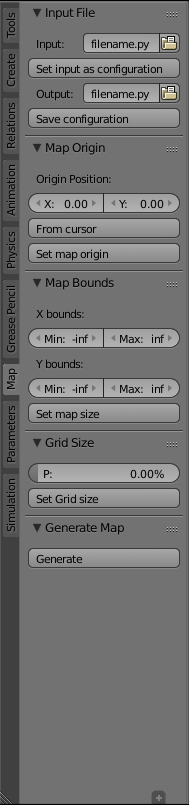
\includegraphics[height=10cm]{img/GUI_map_example.png}
    \caption{Map panel}
  \end{subfigure} % ~
  \begin{subfigure}[t]{0.2\textwidth}
    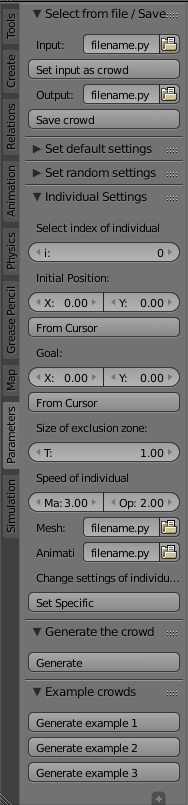
\includegraphics[height=10cm]{img/GUI_crowd_example.png}
    \caption{Crowd panel}
  \end{subfigure} % ~
  \begin{subfigure}[t]{0.5\textwidth}
    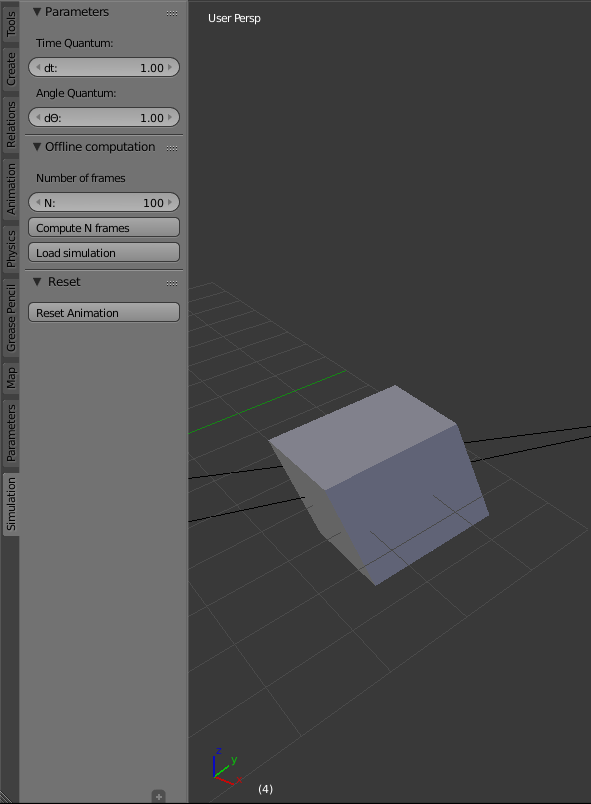
\includegraphics[height=10cm]{img/GUI_simulation_example.png}
    \caption{Simulation panel}
  \end{subfigure}
  \caption{The three panels of the GUI}
\end{figure}
  
\clearpage

\section{Environment plug-in}

\subsection{Overview}

The architecture of the plug-in comes from
\cite{DeclarativeArchitecture}, to provide an intuitive way of
building an environment: by drawing features on a map. The most
difficult part in this approach is that intersecting features are
allowed and should give a result consistent with user expectations.

As a starting point, we focused on generating a height map, using the
concepts from \cite{FeatureTree}. It had the advantage of being able
to merge features smoothly whenever they intersect, rather than using
the more convoluted conflict-resolution mechanism of
\cite{DeclarativeArchitecture}.

\bigskip

The basic unit managed by this plugin is a \emph{feature}, which lies
in a certain area, has a certain height profile and knows how to
interact with the other features that may intersect it. From the
collection of all the features drawn on the map by the user, our
plug-in builds a tree encoding how to build the final height map by
successively merging sets of features together.  %TODO: mention models
(e.g. trees for forests)


\subsection{Features}

\subsubsection{Mountains}

Our first implementation of the Mountain feature corresponded to what
is presented in \cite{FeatureTree}, where mountains are generated
procedurally. However, the 2D random functions we tried did not yield
satisfying results. That's why we switched to another version, where
we import at random a part of a heightmap taken from a website
\cite{terrain-party}. This website import the heightmaps through
satellite imaging.

\subsubsection{Cities}

We planned a feature that could generate cities, following a
three-step process. First, draw the street network. For this task we
chose to use the method of \cite{StreetTensors}, which provides a more
or less intuitive way for the user to control the output. Then, divide
each street-delimited block into parcels. We chose to follow the
approach of \cite{PGParcels}, which seemed to give realistic
results. Finally, put a building in each parcel. We did not look much
into that last part because using buildings of random height was
thought to be a reasonable approximation.

However, even the first step turned out to be challenging to
implement. The principle of the chosen method was to describe the
shape of the street network by a tensor field, mapping points to $2
\times 2$ matrices. It is described by a combination of basic fields
given by the user. The streets are then drawn as the stream lines of
the eigenvectors of the field. The main issue here was to represent
the street network under construction so that:
\begin{itemize}
  \item street drawing starts from points belonging to old streets and
satisfying certain constraints
  \item new intersections are correctly handled while drawing a street
  \item the right eigenvector is always chosen
\end{itemize} without having to reimplement the computation of
eigenvectors or the numerical approximation of a differential
equation.

%% On ne parle pas trop de ce qui allait pas là non ?

\subsection{Graphical User Interface (GUI)}

A picture of the interface is presented in
Fig.~\ref{fig:env-gui1}. Using the interface, the user can choose the
feature he wants to draw. He can then draw it using a pencil
integrated in Blender, drawing polygons here. After having completed
the drawing of the features, the user can ask for the generation of
the environment. It can then hide the polygons, and also modify
parameters that are feature-specific.

\begin{figure}
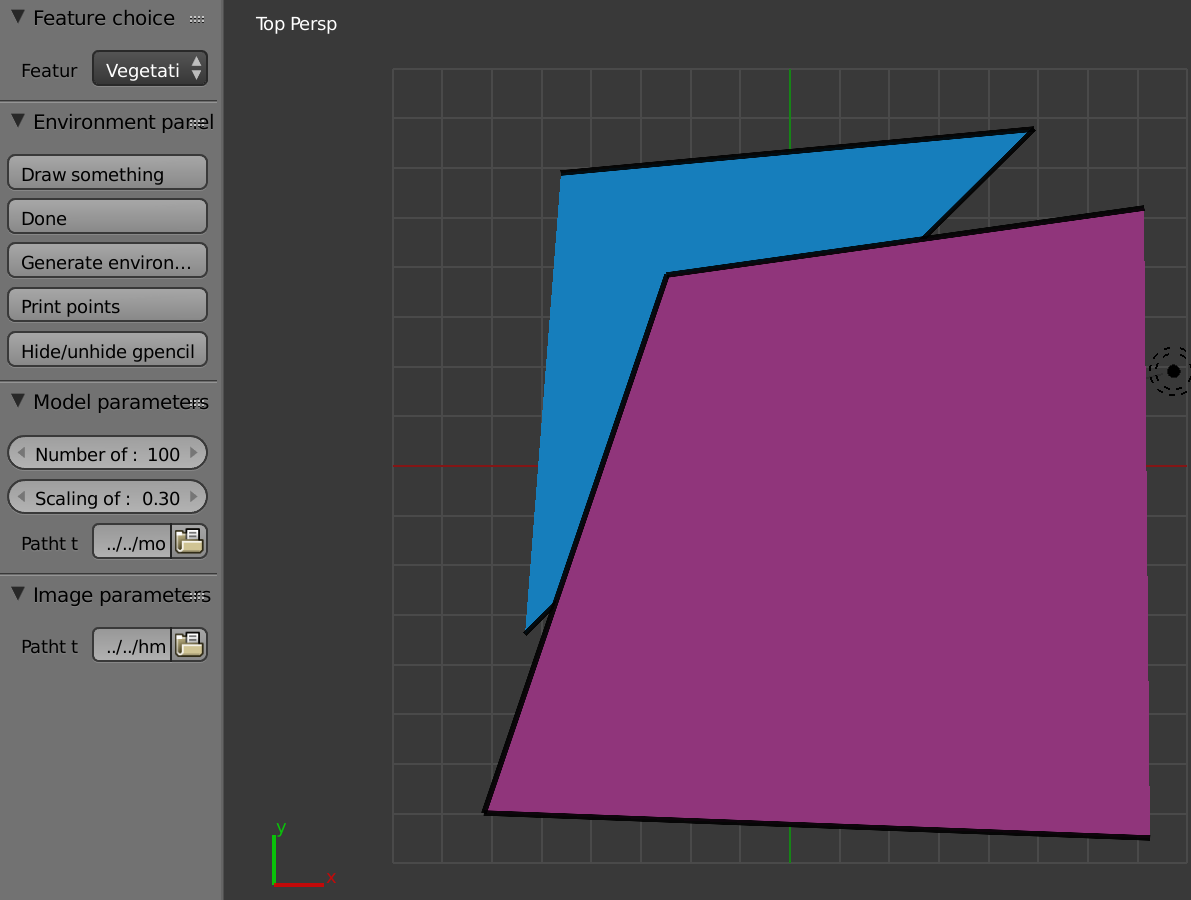
\includegraphics[width=\textwidth]{img/env_gui1.png}
\caption{GUI of the Environment plug-in, with two features (in blue
and magenta)}
\label{fig:env-gui1}
\end{figure}

%% Eventuellement : faire deux images, une du dessin des features, et
%% une de la génération ?

\clearpage

\section{Conclusion}

At the end of this project, we were able to render the following animation using our two plug-ins: \url{blendit.github.io/demo.mp4}. Our global proposal is mainly respected: we are able to generate environments provided by the user in an intuitive way, and we are able to generate crowds where people avoid each other. Thanks to a lot of planning, and to the unitary tests, we did not have any tricky bug to fix during the development of our project. Still, we have been slowed down by some difficulties: we did not realize the animation of individuals would take so much time;  we understood the graph implementation was too computationally expensive too late to try another approach; we also did not had the time to develop as many features as we wished concerning the generation of environments. 

\subsection*{Future work}

Our implementation is functional, but can be improved. Among possible improvements, we could try to make both plug-in interact more. Concerning the crowd simulation part, it would be interesting to develop an efficient version of the control of the path using a graph, and maybe add options to create way-points. Another thing to do is to create an animation for the individuals. Concerning the environment generation, the city feature is not ready yet, and live modifications (going backward to edit a feature) are not supported.




\newpage
\begingroup

\bibliographystyle{ieeetr}
\bibliography{final}

\endgroup

\end{document}
